\begin{tikzpicture}
	\draw[
	-{Triangle[width=24pt,length=18pt]},
	line width=16pt,
	color=\tertiarycolor!30
	] (2.35, 0) -- ++(2.5,0); % relative placement
	\node (c) at (3.5,0) {\bfseries \color{\tertiarycolor} Decoding};

	\begin{scope}
		% clip rectangle: adjust the x value to taste
		\clip (-4.5,-2) --
		(-4.5,2) --
		(3.5,2) --
		(2.8, 1.5) --
		(2.8, -1.2) --
		(2, -1.2) --
		(2, -2) -- cycle;
		\node (qag) at (0,0) {\input{tikz/qag_model2}};
	\end{scope}

	\node (1dshower) at ([xshift=1.25cm, yshift=-.3cm]qag.east)
	{\scalebox{.85}{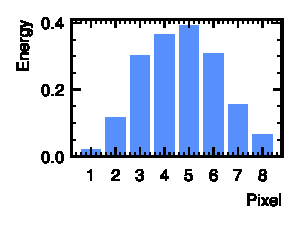
\includegraphics{assets/1Dshow_8_0}}};

	\draw[
		black,
		line width=0.8pt,
		rounded corners=4pt
	]
	([xshift=-.25cm, yshift=-.25cm]current bounding box.south west)
	rectangle
	([xshift=-.15cm, yshift=.75cm]current bounding box.north east);

	\node[anchor=west] at ([xshift=.25cm, yshift=-.35cm]current bounding box.north west) {\bfseries A: Fully Quantum Model};

\end{tikzpicture}